\documentclass[5p]{elsarticle} %review=doublespace preprint=single 5p=2 column
%%% Begin My package additions %%%%%%%%%%%%%%%%%%%
\usepackage[hyphens]{url}

  \journal{An awesome journal} % Sets Journal name

\sloppy

\usepackage{lineno} % add

\usepackage{graphicx}
%%%%%%%%%%%%%%%% end my additions to header

\usepackage[scaled]{helvet}

% Für die Schriftart Helvecia
\renewcommand*\familydefault{\sfdefault} 



\usepackage[T1]{fontenc}
\usepackage{lmodern}
\usepackage{amssymb,amsmath}
\usepackage{ifxetex,ifluatex}
\usepackage{fixltx2e} % provides \textsubscript
% use upquote if available, for straight quotes in verbatim environments
\IfFileExists{upquote.sty}{\usepackage{upquote}}{}
\ifnum 0\ifxetex 1\fi\ifluatex 1\fi=0 % if pdftex
  \usepackage[utf8]{inputenc}
\else % if luatex or xelatex
  \usepackage{fontspec}
  \ifxetex
    \usepackage{xltxtra,xunicode}
  \fi
  \defaultfontfeatures{Mapping=tex-text,Scale=MatchLowercase}
  \newcommand{\euro}{€}
\fi
% use microtype if available
\IfFileExists{microtype.sty}{\usepackage{microtype}}{}
\bibliographystyle{elsarticle-harv}
\ifxetex
  \usepackage[setpagesize=false, % page size defined by xetex
              unicode=false, % unicode breaks when used with xetex
              xetex]{hyperref}
\else
  \usepackage[unicode=true]{hyperref}
\fi
\hypersetup{breaklinks=true,
            bookmarks=true,
            pdfauthor={},
            pdftitle={Exploring an economical approach to the construction of a forest microclimate model},
            colorlinks=false,
            urlcolor=blue,
            linkcolor=magenta,
            pdfborder={0 0 0}}
\urlstyle{same}  % don't use monospace font for urls

\setcounter{secnumdepth}{5}
% Pandoc toggle for numbering sections (defaults to be off)


% tightlist command for lists without linebreak
\providecommand{\tightlist}{%
  \setlength{\itemsep}{0pt}\setlength{\parskip}{0pt}}


% Pandoc citation processing
\newlength{\cslhangindent}
\setlength{\cslhangindent}{1.5em}
\newlength{\csllabelwidth}
\setlength{\csllabelwidth}{3em}
\newlength{\cslentryspacingunit} % times entry-spacing
\setlength{\cslentryspacingunit}{\parskip}
% for Pandoc 2.8 to 2.10.1
\newenvironment{cslreferences}%
  {}%
  {\par}
% For Pandoc 2.11+
\newenvironment{CSLReferences}[2] % #1 hanging-ident, #2 entry spacing
 {% don't indent paragraphs
  \setlength{\parindent}{0pt}
  % turn on hanging indent if param 1 is 1
  \ifodd #1
  \let\oldpar\par
  \def\par{\hangindent=\cslhangindent\oldpar}
  \fi
  % set entry spacing
  \setlength{\parskip}{#2\cslentryspacingunit}
 }%
 {}
\usepackage{calc}
\newcommand{\CSLBlock}[1]{#1\hfill\break}
\newcommand{\CSLLeftMargin}[1]{\parbox[t]{\csllabelwidth}{#1}}
\newcommand{\CSLRightInline}[1]{\parbox[t]{\linewidth - \csllabelwidth}{#1}\break}
\newcommand{\CSLIndent}[1]{\hspace{\cslhangindent}#1}


\usepackage{diagbox}
\usepackage{makecell}

\begin{document}


\begin{frontmatter}

  \title{Exploring an economical approach to the construction of a forest microclimate model}
    \author[Philipps-University Marburg]{Thomas Beier}
   \ead{Beierth@students.uni-marburg.de} 
    \author[Philipps-University Marburg]{Florian Franz}
   \ead{Franzf@students.uni-marburg.de} 
    \author[Philipps-University Marburg]{Konstantin Seeger}
   \ead{Seegerk@students.uni-marburg.de} 
      \address[Philipps-University Marburg]{Philipps-University Marburg,
FB 19 Geography, Deutschhausstraße 10, 35032 Marburg, Germany}
    
  \begin{abstract}
  Forests with their regulation functions are important ecosystems in the context of climate change. In addition to forests functioning as CO2 reservoirs, the canopy can buffer climate extremes such as heat, leading to lower temperatures than outside the forest. This special microclimate provides climatic microrefugia for many species. For identification purposes of such microrefugia, valid models of forest microclimate are needed. In recent years, much attention has been paid to models using predictors derived from Light Detection and Ranging (LiDAR) data and point-based measurements from data loggers as response. However, it is still unclear how many such data loggers are needed for a valid prediction of microclimate. In this study, we explored an economical approach to the construction of a forest microclimate model using LiDAR data to determine a cost-effective model. Our results revealed a decreasing prediction quality with fewer data loggers used for training, but the differences were only small. Considering only the number of data loggers is not useful. A sensible distribution of the station's position in the modeled area is much more important to reflect the different microclimates in the forest.
  \end{abstract}
   \begin{keyword} Microclimate, Economical approach, Treetalker, Temperature, MOF, LiDAR, Random forest classification\end{keyword}
 \end{frontmatter}

\newpage

\hypertarget{introduction}{%
\section{Introduction}\label{introduction}}

\graphicspath{ {./figures/} }

\begin{figure*}[t]
\begin{center}
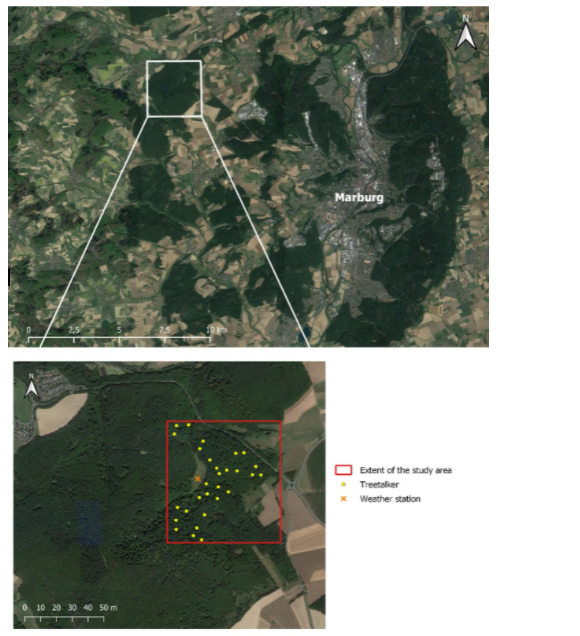
\includegraphics[scale=0.8]{study_area}
\caption{Location of the study area MOF (white square) and extent with locations of the treetalkers and the weather station}
\end{center}
\end{figure*}

The climate within forest stands can differ considerably from that outside forests in free, open landscapes (Bramer et al. 2018, Chen et al. 1999, De Frenne et al. 2019, De Frenne et al. 2021). This microclimate or micrometeorological scale range describes all climatic conditions of an area close to the earth’s surface (Chen et al. 1999), which includes atmospheric processes with a horizontal extension of up to 100 meters (DWD 2022, Foken 2006). Meteorological variables such as temperature, light, wind speed, and moisture (Chen et al. 1999) are strongly influenced by the underlying surface and vegetation cover, promoting forests to create a special microclimate (De Frenne et al. 2019, Zellweger et al. 2020). Depending on the forest structure and canopy cover (Aussenac 2000, Ehbrecht et al. 2019), macroclimate and local water balance (Davis et al. 2019a, De Frenne et al. 2019), forests have the potential to moderate global warming impacts (De Frenne et al. 2019). This buffered microclimate provides climatic microrefugia for many species as macroclimatic extremes increase (Lenoir et al. 2017, Scheffers et al. 2014). Viewing the broad impacts of anthropogenic climate change to biodiversity (Scheffers et al. 2016), it is crucial to identify such climatic microrefugia for possible designation of protected areas (Keppel et al. 2012, Keppel et al. 2015). For this purpose, microclimate models can be helpful, as they allow a spatiotemporal prediction of climatic conditions on a small scale (Frey et al. 2016, Meineri \& Hylander 2017).
Several studies have been conducted on forest microclimate modeling (e.g. Frey et al. 2016, George et al. 2015, Greiser et al. 2018, Vanwalleghem \& Meentemeyer 2009). Machine learning approaches that use a certain number of predictor variables and one or more response variables are widely used in this context (Frey et al. 2016, George et al. 2015, Greiser et al. 2018). Meteorological variables such as temperature or humidity measured by data loggers commonly serve as response variables (Frey et al. 2016), while the predictors often include several structure-describing variables, as forest structural elements have shown to be substantial drivers of microclimate (Kovács et al. 2017). In recent years, remote sensing technologies have significantly enhanced microclimate modeling and mapping due to their ability to measure such structural characteristics of forests, especially using Light Detection and Ranging (LiDAR) systems (Zellweger et al. 2019). LiDAR as active sensors emit laser pulses in the near-infrared spectrum to measure the distance to a target, typically the earth’s surface (Wulder et al. 2008). Aircraft-mounted LiDAR instruments, also known as airborne laser scanning (ALS), and generated 3-dimensional point clouds are highly appropriate for forest research, as they enable an accurate derivation of horizontal and vertical information (Beland et al. 2019, Lim et al. 2003, Wulder et al. 2008, Zellweger et al. 2019). Such LiDAR derived metrics could be, for example, the canopy height, the Leaf Area Index (LAI), or the biomass (Lim et al. 2003, Wulder et al. 2008). Some of these are well suited for stand structure characterization (del Río et al. 2016), and thus for predicting microclimate (Davis et al. 2019b, Zellweger et al. 2019).
Despite the widespread approach of using point-based measurements as response variables, it still remains an open question how many such points (or data loggers) are needed for a valid prediction of microclimate. However, a cost-effective model would require knowledge of the minimum number of such measurement points. Hence, we explored an economical approach to the construction of a forest microclimate model for the Marburg Open Forest (MOF) near the city of Marburg (Hesse, Germany). Our objective was to determine the minimum number of point measurement stations for a valid prediction of the temperature in the forest. We further investigated how the omission of stations affected the prediction of other stations. Our results may provide useful information for future studies on microclimate modeling, when it may be possible to conduct them in a more cost-effective way.


\hypertarget{materials-and-methods}{%
\section{Materials and Methods}\label{materials-and-methods}}

\hypertarget{study-area}{%
\subsection{\texorpdfstring{Study area\\
}{Study area }}\label{study-area}}

The study was conducted in the ‘Calderner Forst’ referred to as MOF because of its proximity (7 km northeast) to the city of Marburg (Fig. 1). It is roughly located on 50° 50’ 25.8’’ N and 8° 40’ 59.52’’ E with elevation ranges between 233 m and 411 m above sea level. It is a mixed forestry stand that is also used for various research activities, which can draw on a network of different operated sensors. The forest is mainly dominated by beech, oak, alder, spruce, and a meadow. This study was focussed on an extent of the MOF in the northeast (Fig. 1), covering an area of 55 ha.


\hypertarget{data}{%
\subsection{\texorpdfstring{Data\\
}{Data }}\label{data}}

LiDAR data was provided by the “Hessische Landesamt für Naturschutz, Umwelt und Geologie” (HLNUG). The aerial survey was done in spring 2018 under leaf off conditions with a \emph{Riegl LMS-Q780} sensor. LiDAR data was used for the extent of the red square in Fig. 1. In the MOF there are 100 treetalker stations (TT+ 3.3 version, NATURE 4.0 SB SRL 2022) from which 29 are located in the extent of our study area (Fig. 1). However, in the period we studied, from June to August 2020, data was only available for 18 of them. In addition to various measurements of tree functions they record temperature and humidity from which temperature was used. Additionally to the treetalker stations, a weather station standing on the meadow in the MOF was also used. The weather station records more than 30 climate components and started operating in June 2017. The exact position is also visible in Fig. 1.


\hypertarget{predictors}{%
\subsection{\texorpdfstring{Predictors\\
}{Predictors }}\label{Predictors}}

We used the \emph{lidR} package by Roussel et al. (2022) for processing LiDAR data in the programming language R (R Core Team 2022). Generally, all coding was performed in RStudio (R Core Team 2022). 
For the extent of the study area, 67 predictors derived from the LiDAR data were calculated on 1 meter grid level. These predictors can be found in Tab. 1. To calculate them, we first applied a point cloud normalization using inverse distance weighting as an algorithm for spatial interpolation (Roussel et al. 2021, Roussel et al. 2020). 56 out of these 67 predictors are part of the standard metrics in the \emph{lidR} package. The standard metrics are a collection of several commonly used statistical metrics like the mean height, mean intensity, and many other metrics (Roussel et al. 2022). The Canopy Height Model (CHM) was calculated with a pit-free algorithm (Khosravipour et al. 2014), including 2, 5, 10, and 15 m as height thresholds for triangulations of first returns and a maximum edge of 1.5 (Roussel et al. 2021, Roussel et al. 2020). The Leaf Area Index (LAI) was calculated using the \emph{canopyLazR} package (Kamoske et al. 2019). We used inverse distance weighting again for generating a Digital Terrain Model (DTM), including 6 closest neighbours and a power of 2 (Roussel et al. 2021, Roussel et al. 2020). The DTM was further used to calculate the slope, aspect, and Topographic Position Index (TPI) with corresponding built-in functions in the \emph{raster} package by Hijmans et al. (2022). The first return metrics as well as point and pulse density were calculated with self-defined and pre-definded functions found in Roussel et al. (2021). Many of the 67 predictors have already been proven in other studies for predicting microclimate (e.g. Carrasco et al. 2019, Bennie et al 2008, Hardiwck et al. 2014). A good overview can be found in Carrascon et al. (2019), who provided a correlation matrix among LiDAR derived metrics and temperature. But because all of these predictors were static a real prediction couldn’t be made. Hence, 28 climate variables obtained by the weather station located on the meadow within the forest were also used as predictors.

\hypertarget{model creation and validation}{%
\subsection{\texorpdfstring{Model creation and validation\\
}{Model creation and validation }}\label{model-creation-and-validation}}

All the LiDAR predictors were stacked in a rasterStack using the \emph{raster} package. Afterwards, the pixel information of all the treetalker stations in the rasterStack were extracted into a data frame for every possible hour in the examination period. The hourly values of the climate variables were also added to the data frame. Next step was to remove NA-values and balance the data so that from every station the same amount of data was used. This was done to avoid bias. The cleaning of the data frame continued by removing near-zero values and correlated predictors with a cutoff value of 0.9. 
For validation purposes, the data frame was split in a 80 to 20 ratio in training and test data using the caret package (Kuhn et al. 2022). The pixel-point of the weather station on the meadow was used as independent data to also validate the different models. Next a function was created that could randomly remove a specified amount of stations, calculate a machine learning random forest ranger model from the remaining stations, predict the temperature and calculate the root-mean-square error (RMSE) for each station and the weather station. The results of each model run were cross-validated three times to create more accurate predictions. Hyperparameter tuning was applied to the model with the combination of \emph{mtry} = 5 to 10, \emph{splitrule} = “extratrees” and \emph{min.node.size} = 5,10 or 15. The function was used five times to remove one station, five times to remove two stations and so on until 17 stations, the most possible, were five times removed. In addition, a model with all the stations included in the training data was calculated to compare it to the results where stations were removed. Based on the results of the RMSE of the climate station and the treetalker stations, the aim of this study was evaluated. 

\begin{table}[!h]
\renewcommand{\arraystretch}{2}
\begin{center}
\caption{LiDAR-derived metrics used as predictors.}
\scalebox{0.8}{
 \begin{tabular}{l  l  c  l} 
 \hline
 \\
 \textbf{Name} & \textbf{References} \\ [1ex]
 \hline
 CHM & Carrasco et al. 2019 \\ [1.5ex]
 
 First return metrics (mean/max/std) & Carrasco et al. 2019 \\ [1.5ex]

 Point density & Roussell et al. 2021 \\ [1.5ex]

 Pulse density & Roussell et al. 2021 \\ [1.5ex]
 
 LAI & \makecell[l]{Hardwick et al. 2014,\\ 
 Roth et al. 2020,\\ 
 Kamoske et al. 2019} \\ [1.5ex]
 
 DTM & \makecell[l]{George et al. 2015,\\ Latif 2012} \\ [1.5ex]
 
 Slope & Bennie et al. 2008 \\ [1.5ex]
 
 Aspect & Bennie et al. 2008 \\ [1.5ex]
 
 TPI & Ivajnšič et al. 2014 \\ [1.5ex]
 
 Standard metrics & Roussell et al. 2021 \\ [1.5ex]
 
 \hline
 \end{tabular}}
 \end{center}
\end{table}

\hypertarget{results}{%
\section{Results}\label{results}}

After cleaning the data frame, only 46 predictors remained. 11 of them were from the climate station on the meadow and the rest were LiDAR predictors. 

\begin{figure}[!ht]
\begin{center}
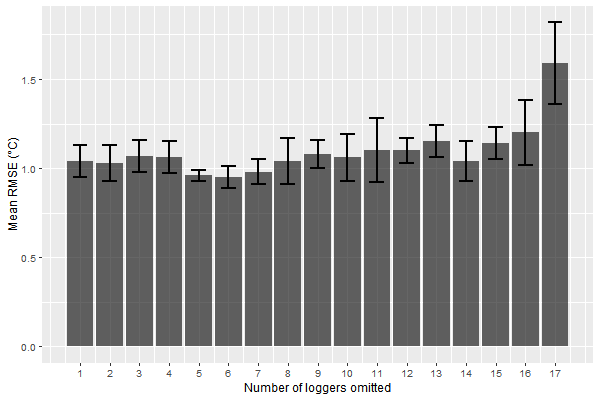
\includegraphics[scale=0.48]{rmse_wiese_mean_barplot}
\caption{Mean RMSE with error bars calculated for the weather station on the meadow.}
\end{center}
\end{figure}

\begin{figure}[!h]
\begin{center}

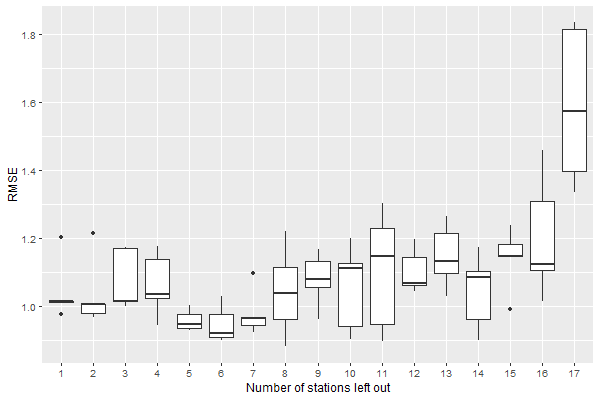
\includegraphics[scale = 0.48]{rmse_wiese_boxplot}
\caption{Boxplots of the RMSE calculated for the weather station on the meadow.}
\end{center}
\end{figure}

The results of all the model runs with decreasing number of stations are shown in Fig. 2 and 3. Fig. 2 shows the mean RMSE from the independent weather station of all the different models runs. In addition, the standard deviation is shown. Fig 3. shows the same but as boxplots. Generally, both figures show that with less stations removed the predictions were better than having many stations removed. But the difference between leaving 1 or 2 stations out, to leaving 13 or 14 stations out was not huge. In fact when removing 5, 6 or 7 stations, the mean and the median RMSE were best with a value less than 1.0, while removing 1 or 2 stations led to a mean and median RMSE of higher than 1.0. The boxplot shows that with 14 or 15 removed stations, a RMSE with a value less than 1.0 was possible to be achieved. Only when 17 stations were removed, a clear drop in the RMSE performance was visible.
When taking a look at all the 85 function runs, we noticed that the 19 best performing function runs according to the RMSE of the weather station removed all at least 4 stations. The 20th run was the first one that removed less than 4 stations. On the other side, in the worst twenty runs it was three times the case that less than four stations were removed. 
Fig. 4 evaluates the performance of the mean RMSE of each treetalker station with an increasing number of left out treetalker stations. As with the weather station, the RMSE increased with the number of stations left out. The best performing stations had RMSE values of around 0.4 when just one or two stations were removed. It is once again visible that even with 13, 14 or 15 stations left out some of the stations were still having a relatively good RMSE of around 0.8. It is also clearly evident that only around half of the stations performed well, while the rest had problems predicting temperature and had slightly worse or way worse RMSE values even with one station left out. Especially the treetalker stations 12 and 28 revealed problems in predicting temperature. Both of them had a RMSE value of around 1.0 with just one station left out but were able to hold this consistent RMSE value if less than eight stations were removed.
To further evaluate how the predictions perform, we predicted for one hour the temperature of each number of left out stations for the study area. The results can be found in Fig. 5. The predictions were done for 12/06/2020 at 18:00. With a low number of removed stations the predictions have pixels that reach temperature close to  22 °C, meanwhile with a high number of removed stations the predictions are way lower and have problems even reaching  21 °C. When removing 17 stations it appears that for the whole study area each pixel is predicted with the same value. 




\begin{figure*}[h]
\begin{center}
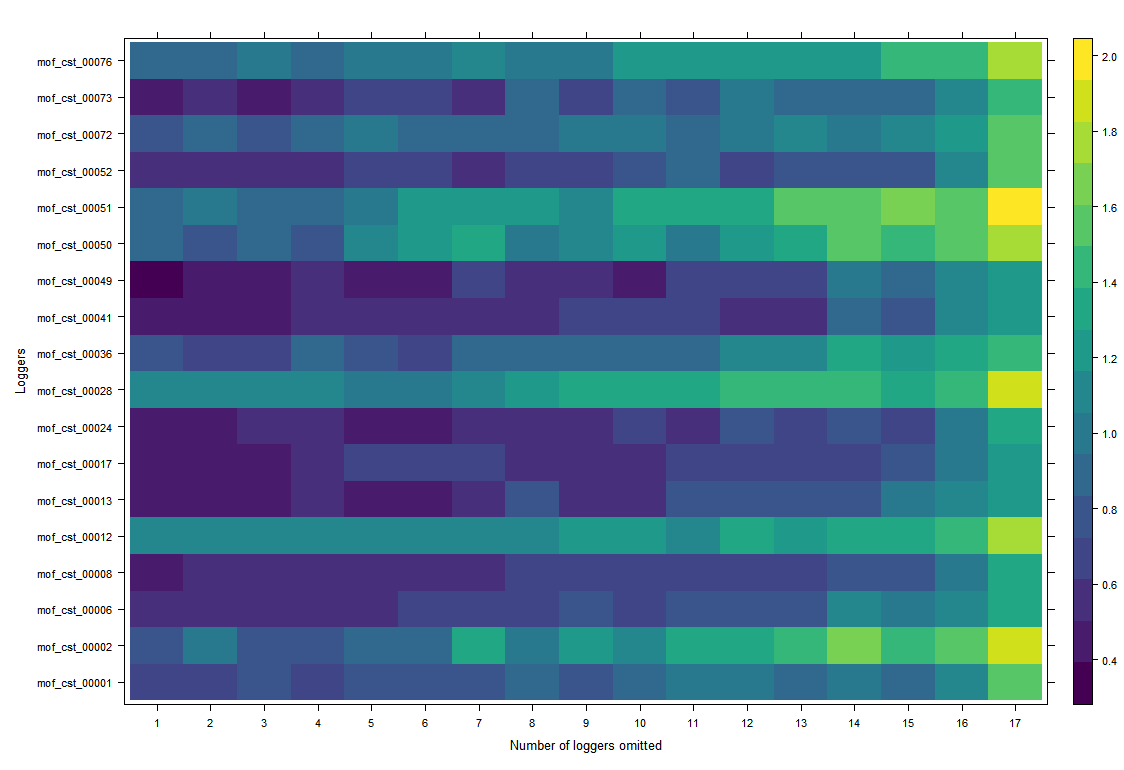
\includegraphics[scale=0.5]{heatmap_treetalker_rmse}
\caption{RMSE change of each treetalker with increasing number of removed treetalker stations.}
\end{center}
\end{figure*}

\begin{figure*}[t]
\begin{center}
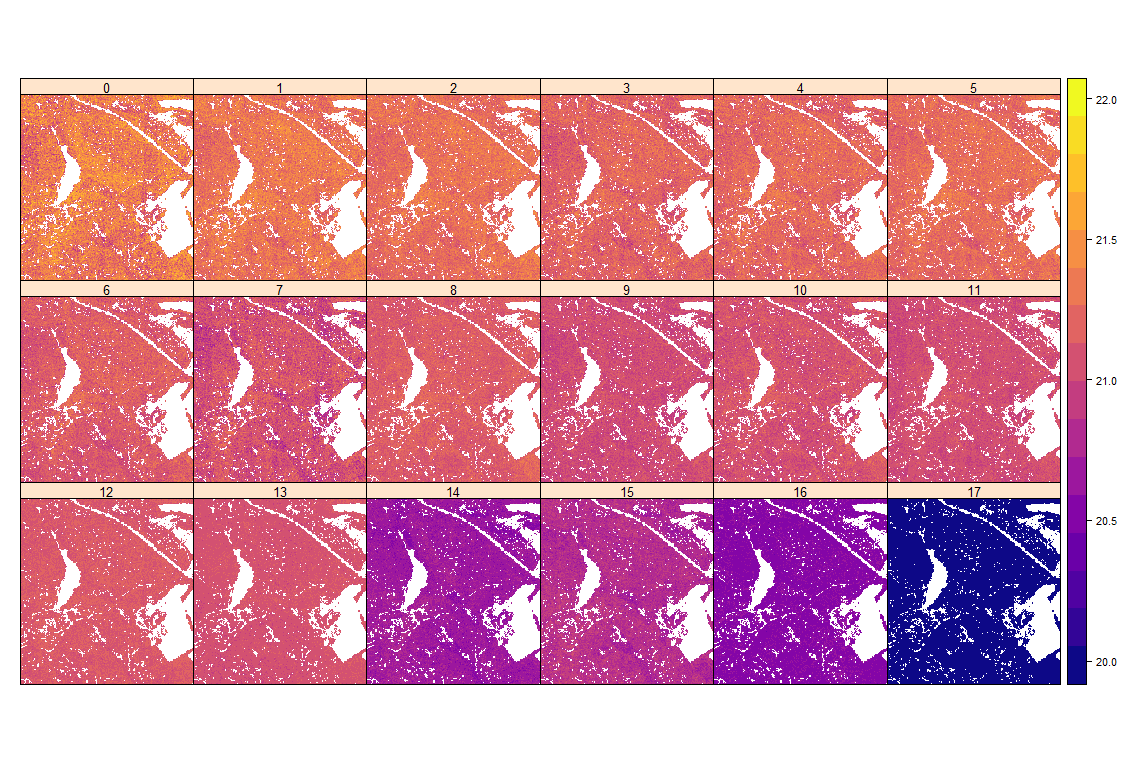
\includegraphics[scale=0.5]{full_prediction_study_area}
\caption{Temperature (°C) prediction of the study area for 12/06/2020 at 18:00. With an increasing number of left out stations.}
\end{center}
\end{figure*}

\hypertarget{discussion}{%
\section{Discussion}\label{discussion}}

Predicting forest microclimate using different machine learning approaches is a widely used method applied in several forest types of the world (e.g. Frey et al. 2016, George et al. 2015, Greiser et al. 2018). In recent years, studies have highlighted the benefits of remote sensing technologies for such tasks, especially the use of LiDAR (Frey et al. 2016, Zellweger et al. 2019). We applied a similar approach, using airborne LiDAR data to derive common metrics for predicting temperature in a mixed forestry stand. However, we have further investigated the extent to which the omission of stations influences the prediction results.
Our results revealed a decreasing prediction quality with an increasing number of stations left out. However, this does not mean that a higher number of stations generally improves the prediction. The RMSE values between few omitted stations (1 or 2) and more omitted stations (13 or 14) differed by only about 0.2. Only when 17 stations were left out, meaning only one station was used for model training, a more significant decrease in the RMSE was noticeable. Hence, the selection of the station's position seems to be much more important than the number of stations. This was shown by the RMSE change at the individual stations with an increasing number of removed stations (Fig. 4). While several stations performed well in predicting temperature even if up to 15 stations were left out, some showed a worse prediction. This was particularly evident for treetalker stations 12 and 28. The predictor values on these two stations seem to be most optimal for a valid prediction of temperature in our study area. The best function runs always occurred when stations 12 and 28 were included or only one of them was omitted. This also explains the high RMSE values even if 14 or 15 stations were left out. Therefore, it does not necessarily require many stations, rather a sensible distribution of these in the modeled area to reflect the different microclimates in the forest. It needs to be added that there is a small bias because only 5 different combinations were run for each amount of removals. More function runs could have been made but especially the running time when only removing a low number of stations took a lot of time.


\hypertarget{conclusion}{%
\section{Conclusion}\label{conclusion}}

Here comes the text for the conclusion

\hypertarget{references}{%
\section*{References}\label{references}}
\addcontentsline{toc}{section}{References}

\hypertarget{refs}{}
\begin{CSLReferences}{1}{0}


Beland, M., Parker, G., Sparrow, B., Harding, D., Chasmer, L., Phinn, S., Antonarakis, A. \& Strahler, A. (2019): On promoting the use of lidar systems in forest ecosystem research. \emph{For. Ecol. Manag.} 450, 117484.

Bennie, J., Huntley, B., Wilshire, A., O.Hill, M. \& Baxter R. (2008): Slope, aspect and climate: Spatially explicit and implicit models of topographic microclimate in chalk grassland. \emph{Ecol. Model.} 216 (1), 47-59.

Bramer, I., Anderson, B.J., Bennie, J., Bladon, A.J., De Frenne, P., Hemming, D., Hill, R.A., Kearney, M.R., Körner, C., Korstjens, A.H., Lenoir, J., Maclean, I.M.D., Marsh, C.D., Morecroft, M.D., Ohlemüller, R., Slater, H.D., Suggitt, A.J., Zellweger, F. \& Gillingham, P.K. (2018): Advances in monitoring and modelling climate at ecologically relevant scales. In: Bohan, D.A., Dumbrell, A.J., Woodward, G. \& Jackson, M. (Eds.): \emph{Adv. Ecol. Res.} 58. Next generation biomonitoring: part 1., 101-161.

Carrasco, L., Giam, X., Papeş, M. \& Sheldon, K.S. (2019): Metrics of Lidar-Derived 3D Vegetation Structure Reveal Contrasting Effects of Horizontal and Vertical Forest Heterogeneity on Bird Species Richness. \emph{Remote Sens.} 11 (7), 743.

Chen, J., Saunders, S.C., Crow, T.R., Naiman, R.J., Brosofske, K.D., Mroz, G.D., Brookshire, B.L. \& Franklin, J.F. (1999): Microclimate in Forest Ecosystem and Landscape Ecology. Variations in local climate can be used to monitor and compare the effects of different management regimes. \emph{BioScience} 49 (4), 288-297.

Davis, K.T., Dobrowski, S.Z., Holden, Z.A., Higuera, P.E. \& Abatzoglou, J.T. (2019a): Microclimatic buffering in forests of the future: the role of local water balance. \emph{Ecography} 42 (1), 1-11.

Davis, F.W., Synes, N.W., Fricker, G.A., McCullough, I.M., Serra-Diaz, J.M., Franklin, J. \& Flint, A.L. (2019b): LiDAR-derived topography and forest structure predict fine-scale variation in daily surface temperatures in oak savanna and conifer forest landscapes. \emph{Agric. For. Meteorol.} 269-270, 192-202.

De Frenne, P., Zellweger, F., Rodríguez-Sánchez, F., Scheffers, B.R., Hylander, K., Luoto, M., Vellend, M., Verheyen, K. \& Lenoir, J. (2019): Global buffering of temperatures under forest canopies. \emph{Nat. Ecol. Evol.} 3, 744-749.

De Frenne, P., Lenoir, J., Luoto, M., Scheffers, B.R., Zellweger, F., Aalto, J., Ashcroft, M.B., Christiansen, D.M., Decocq, G., Pauw, K.D., Govaert, S., Greiser, C., Gril, E., Hampe, A., Jucker, T., Klinges, D.H., Koelemeijer, I.A., Lembrechts, J.J., Marrec, R., Meeussen, C., Ogée, J., Tyystjärvi, V., Vangansbeke, P. \& Hylander, K. (2021): Forest microclimates and climate change: Importance, drivers and future research agenda. \emph{Glob. Change Biol.} 27 (11), 2279-2297.

Deutscher Wetterdienst (DWD) (2022): Mikroklima. \url{https://www.dwd.de/DE/service/lexikon/Functions/glossar.html?lv2=101640&lv3=101778} (Accessed on 2022/03/28).

Foken, T. (2006): Angewandte Meteorologie. Mikrometeorologische Methoden. 2. Auflage. Springer-Verlag. Berlin, Heidelberg.

Frey, S.J.K., Hadley, A.S., Johnson, S.L., Schulze, M., Jones, J.A. \& Betts, M.G. (2016): Spatial models reveal the microclimatic buffering capacity of old-growth forests. \emph{Sci. Adv.} 2 (4), e1501392.

George, A.D., Thompson, F.R. \& Faaborg, J. (2015): Using LiDAR and remote microclimate loggers to downscale near-surface air temperatures for site-level studies. \emph{Remote Sens.} Lett. 6 (12), 924-932.

Greiser, C., Meineri, E., Luoto, M., Ehrlén, J. \& Hylander, K. (2018): Monthly microclimate models in a managed boreal forest landscape. \emph{Agric. For. Meteorol.} 250-251, 147-158.

Hardwick, S.R., Toumi, R., Pfeifer, M., Turner, E.C., Nilius, R. \& Ewers R.M. (2014): The relationship between leaf area index and microclimate in tropical forest and oil palm plantation: Forest disturbance drives changes in microclimate. \emph{Agric. For. Meteorol.} 201, 187-195.

Hijmans, R.J., van Etten, J., Sumner, M., Cheng, J., Baston, D., Bevan, A., Bivand, R., Busetto, L., Canty, M., Fasoli, B., Forrest, D., Ghosh, A., Golicher, D., Gray, J., Greenberg, J.A., Hiemstra, P., Hingee, K., Ilich, A., Institute for Mathematics Applied Geosciences, Karney, C., Mattiuzzi, M., Mosher, S., Naimi, B., Nowosad, J., Pebesma, E., Lamigueiro, O.P., Racine, E.B., Rowlingson, B., Shortridge, A., Venables, Bill. \& Wueest, R. (2022): raster: Geographic Data Analysis and Modelling. R package version 3.5-11. \url{https://cran.r-project.org/web/packages/raster/index.html} (Accessed on 31/03/2022).

Ivajnšič, D., Kaligarič M. \& Žiberna I. (2014): Geographically weighted regression of the urban heat island of a small city. \emph{Appl. Geogr.} 53, 341-353. 

Kamoske, A.G., Dahlin, K.M., Shawn, M.D \& Serbin, C.S. (2019): Leaf area density from airborne LiDAR: Comparing sensors and resolutions in a temperate broadleaf forest ecosystem. \emph{For. Ecol. Manag.} 433, 364-375.

Keppel, G., Van Niel, K.P., Wardell-Johnson, G.W., Yates, C.J., Byrne, M., Mucina, L., Schut, A.G.T., Hopper, S.D. \& Franklin, S.E. (2012): Refugia: identifying and understanding safe havens for biodiversity under climate change. \emph{Global Ecol. Biogeogr.} 21 (4), 393-404.

Keppel, G., Mokany, K., Wardell-Johnson, G.W., Phillips, B.L., Welbergen, J.A. \& Reside, A.E. (2015): The capacity of refugia for conservation planning under climate change. \emph{Front. Ecol. Environ.} 13 (2), 106-112.

Khosravipour, A., Skidmore, A.K., Isenburg, M., Wang, T. \& Hussin, Y.A. (2014): Generating Pit-free Canopy Height Models from Airborne Lidar. \emph{Photogramm. Eng. Remote Sens.} 80 (9), 863–872.

Kovács, B., Tinya, F. \& Ódor, P. (2017): Stand structural drivers of microclimate in mature temperate mixed forests. \emph{Agric. For. Meteorol.} 234-235, 11-21.

Kuhn, M., Wing, J., Weston, S., Williams, A., Keefer, C., Engelhardt, A., Cooper, T., Mayer, Z., Kenkel, B., R Core Team, Benesty, M., Lescarbeau, R., Ziem, A., Scrucca, L., Tang, Y., Candan, C. \& Hunt T. (2022):  caret: Classification and Regression Training. \url{https://cran.r-project.org/web/packages/caret/index.html} (Accessed on 31/03/2022).
 
Latif, Z.A. (2012): Forest Microclimate Modelling Using Remotely Sensed Data. \emph{ISrJ.} 2 (1), 19-25.

Lenoir, J., Hattab, T. \& Pierre, G. (2017): Climatic microrefugia under anthropogenic climate change: implications for species redistribution. \emph{Ecography} 40 (2), 253-266.

Lim, K., Treitz, P., Wulder, M., St-Onge, B. \& Flood, M. (2003): LiDAR remote sensing of forest structure. \emph{Prog. Phys. Geogr.} 27 (1), 88-106.

Meineri, E. \& Hylander, K. (2017): Fine-grain, large-domain climate models based on climate station and comprehensive topographic information improve microrefugia detection. \emph{Ecography} 40 (8), 1003-1013.

NATURE 4.0 SB SRL (2022): NATURE 4.0. Wireless systems for environment, agriculture and wildlife. \url{https://www.nature4shop.com/} (Accessed on 04/04/2022).

R Core Team (2022): The R Project for Statistical Computing. https://www.r-project.org/ (Accessed on 30/03/2022). 

Roth, D.B., Goodenough, A.A.,Brown, S.D., van AArdt, J.A., Saunders, M.G. \& Krause K. (2020): Simulations of Leaf BSDF Effects on Lidar Waveforms. \emph{Remote Sens.} 12 (18), 2909.

Roussel, J.-R., Auty, D., Coops, N.C., Tompalski, P., Goodbody, T.R.H., Sánchez Meador, A., Bourdon, J.-F., De Boissieu, F. \& Achim, A. (2020): lidR: An R package for analysis of Airborne Laser Scanning (ALS) data. \emph{Remote Sens. Environ.} 251, 112061.

Roussel, J.-R., Goodbody, T.R.H. \& Tompalski, P. (2021): The lidR package. \url{https://r-lidar.github.io/lidRbook/index.html} (Accessed on 29/03/2022).

Roussel, J.-R., Auty, D., De Boissieu, F., Sánchez Meador, A., Bourdon, J.-F., Demetrios, G., Steinmeier, L. \& Adaszewski, S. (2022): Package ‘lidR’. \url{https://cran.r-project.org/web/packages/lidR/index.html} (Accessed on 29/03/2022).

Scheffers, B.R., Edwards, D.P., Diesmos, A., Williams, S.E. \& Evans, T.A. (2014): Microhabitats reduce animal’s exposure to climate extremes. \emph{Glob. Change Biol.} 20 (2), 495-503.

Scheffers, B.R., De Meester, L., Bridge, T.C.L., Hoffmann, A.A., Pandolfi, J.M., Corlett, R.T., Butchart, S.H.M., Pearce-Kelly, P., Kovacs, K.M., Dudgeon, D., Pacifici, M., Rondinini, C., Foden, W.B., Martin, T.G., Mora, C., Bickford, D. \& Watson, J.E.M. (2016): The broad footprint of climate change from genes to biomes to people. \emph{Science} 354 (6313), aaf7671.

Vanwalleghem, T. \& Meentemeyer, R.K. (2009): Predicting Forest Microclimate in Heterogeneous Landscapes. \emph{Ecosystems} 12 (7), 1158-1172.

Wulder, M.A., Bater, C.W., Coops, N.C., Hilker, T. \& White, J.C. (2008): The role of LiDAR in sustainable forest management. \emph{For. Chron}. 84 (6), 807-826.

Zellweger, F., De Frenne, P., Lenoir, J., Rocchini, D. \& Coomes, D. (2019): Advances in Microclimate Ecology Arising from Remote Sensing. \emph{Trends Ecol. Evol.} 34 (4), 327-341.

Zellweger, F., De Frenne, P., Lenoir, J., Vangansbeke, P., Verheyen, K., Bernhardt-Römermann, M., Baeten, L., Hédl, R., Berki, I., Brunet, J., Van Calster, H., Chudomelová, M., Decocq, G., Dirnböck, T., Durak, T., Heinken, T., Jaroszewicz, B., Kopecký, M., Máliš, F., Macek, M., Malicki, M., Naaf, T., Nagel, T.A., Ortmann-Ajkai, A., Petřík, P., Pielech, R., Reczyńska, K., Schmidt, W., Standovár, T., Świerkosz, K., Teleki, B., Vild, O., Wulf, M. \& Coomes, D. (2020): Forest microclimate dynamics drive plant responses to warming. \emph{Science} 368, 772-775.


\end{CSLReferences}

\end{document}
